\section{Frequency Blending}

In order to blend the images using the frequency domain, we convert the masked image to the frequency domain and focus on approaches to combine these frequency domains images. We consider 6 ideas of combination. 

\begin{itemize}
\item The first one is named "left-right", this method takes a left half of the first frequency domain image and the right half of the another. The results of this method are shown in figure \ref{fig:left-right}. These images shows a successful combination of the original images but the intersection point is not as smooth as it would be expected, this is because in the frequency domain it is not possible to smooth just a small part of the image (e.g. intersection points), the alternative of blurring (e.g. taking out low frequencies) before applying the left-right blend would end up in the same result but blurred in the whole image and not just the intersection points.

\begin{figure}[h!]
\centering
\begin{subfigure}{0.4\textwidth}
  \centering
  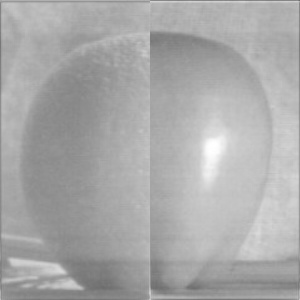
\includegraphics[width=0.7\linewidth]{output/left_right1.jpg}
  \caption{Left-right blending apple-orange}
\end{subfigure}%
\begin{subfigure}{0.4\textwidth}
  \centering
  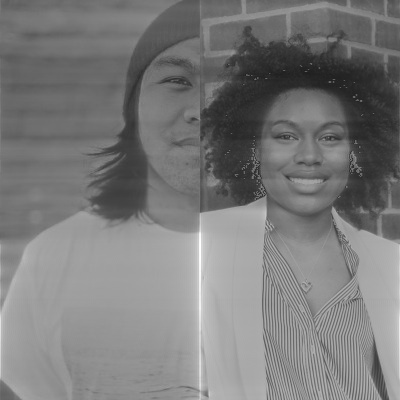
\includegraphics[width=0.7\linewidth]{output/left_right2.jpg}
  \caption{Left-right blending woman-man}
\end{subfigure}%
\caption{Left-right blending}
\label{fig:left-right}
\end{figure}

\item The second method is named "bottom-up", this is similar to the "left\_right" approach but takes the up half of one image and the bottom half of the another. The results of this method are shown in figure \ref{fig:bottom_up}. As equal to the previous approach, the images were successfully joined but with a sharp change in the intersection. Different from previous approach, some vertical shadows appear (left-right approach has horizontal shadows), this highlights the intersection change.

\begin{figure}[h!]
\centering
\begin{subfigure}{0.4\textwidth}
  \centering
  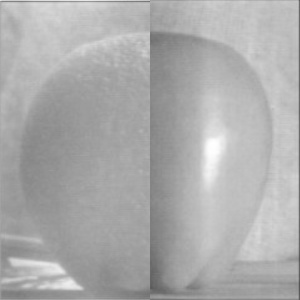
\includegraphics[width=0.7\linewidth]{output/bottom_up1.jpg}
  \caption{Bottom-up blending apple-orange}
\end{subfigure}%
\begin{subfigure}{0.4\textwidth}
  \centering
  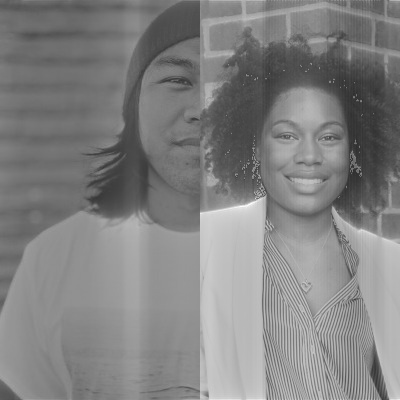
\includegraphics[width=0.7\linewidth]{output/bottom_up2.jpg}
  \caption{Bottom-up blending woman-man}
\end{subfigure}%
\caption{Bottom-up blending}
\label{fig:bottom_up}
\end{figure}

\item The third method is named "centered", this takes the lowest frequencies from one image and the highest frequencies from the other. The results of this method are shown in figure \ref{fig:centered}. Different from previous methods, this approach can not joint the images correctly, it generates a strange combination, this happens because we are taking the lowest frequencies of the second image. Note that in the second combination, the low frequency part is more visible, this due to the quantities of low frequencies that woman image contains.

\begin{figure}[h!]
\centering
\begin{subfigure}{0.4\textwidth}
  \centering
  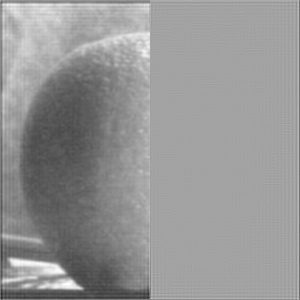
\includegraphics[width=0.7\linewidth]{output/centered1.jpg}
  \caption{Centered blending apple-orange}
\end{subfigure}%
\begin{subfigure}{0.4\textwidth}
  \centering
  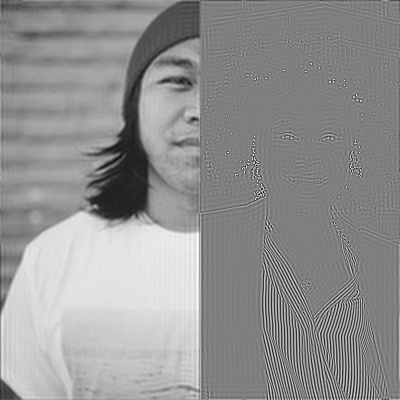
\includegraphics[width=0.7\linewidth]{output/centered2.jpg}
  \caption{Centered blending woman-man}
\end{subfigure}%
\caption{Centered blending}
\label{fig:centered}
\end{figure}

\item The fourth method is named 'chessboard', it combines the frequency images taking one pixel from one image and the next from the other, this creates a kind of chessboard of the frequency images. The results of this method are shown in figure \ref{fig:chessboard}. Due the extreme combination of frequency images, the characteristics of the images mix up generating shadows and photographic negatives.

\begin{figure}[h!]
\centering
\begin{subfigure}{0.4\textwidth}
  \centering
  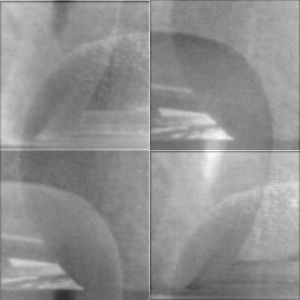
\includegraphics[width=0.7\linewidth]{output/chessboard1.jpg}
  \caption{Chessboard blending apple-orange}
\end{subfigure}%
\begin{subfigure}{0.4\textwidth}
  \centering
  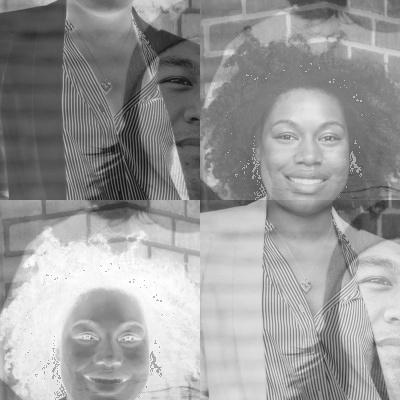
\includegraphics[width=0.7\linewidth]{output/chessboard2.jpg}
  \caption{Chessboard blending woman-man}
\end{subfigure}%
\caption{Chessboard blending}
\label{fig:chessboard}
\end{figure}

\item The fifth method is named "sliding-rows", this creates horizontal stripes intercalating values from the both frequency images. The results of this method are shown in figure \ref{fig:sliding-rows}. These results are interesting because the same method gives really different results, in the case of the apple-orange blending the left side of the image look like a kind of texture of the image (something like a local binary pattern), and the woman-man blending is much more better, the explanation for this effect may be related with the properties of the images, as equal as is centered blending.

\begin{figure}[h!]
\centering
\begin{subfigure}{0.4\textwidth}
  \centering
  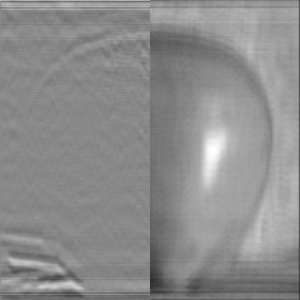
\includegraphics[width=0.7\linewidth]{output/sliding_rows1.jpg}
  \caption{Sliding-rows blending apple-orange}
\end{subfigure}%
\begin{subfigure}{0.4\textwidth}
  \centering
  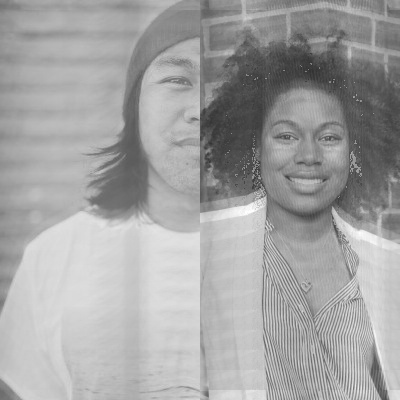
\includegraphics[width=0.7\linewidth]{output/sliding_rows2.jpg}
  \caption{Sliding-rows blending woman-man}
\end{subfigure}%
\caption{Sliding-rows blending}
\label{fig:sliding-rows}
\end{figure}

\item The sixth method is named "sliding-columns", this creates vertical stripes intercalating values from the both frequency images. The results of this method are shown in figure~\ref{fig:sliding-columns}. The experiments looks similar to the previous approach but in this case the images are a little bit more lighter.

\begin{figure}[h!]
\centering
\begin{subfigure}{0.4\textwidth}
  \centering
  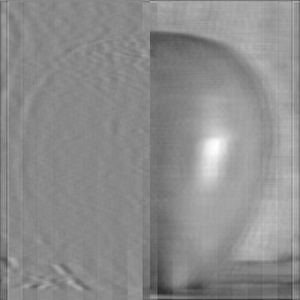
\includegraphics[width=0.7\linewidth]{output/sliding_columns1.jpg}
  \caption{Sliding-columns blending apple-orange}
\end{subfigure}%
\begin{subfigure}{0.4\textwidth}
  \centering
  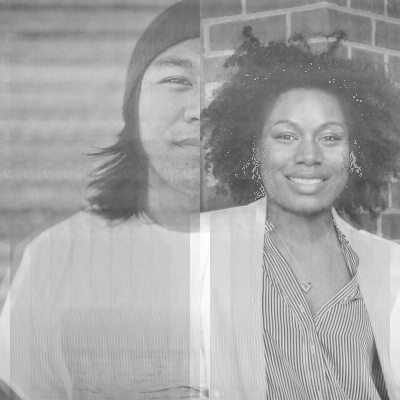
\includegraphics[width=0.7\linewidth]{output/sliding_columns2.jpg}
  \caption{Sliding-columns blending woman-man}
\end{subfigure}%
\caption{Sliding-columns blending}
\label{fig:sliding-columns}
\end{figure}

\end{itemize}

Comparing this results with the obtained in the space domain (figure~\ref{fig:comparison-blending}) we can see that the change in the space domain is smoother, this is because the blending in the frequency domain is not fully development. Note that the frequency domain blending only considers grayscale image as inputs.

\begin{figure}[h!]
\centering
\begin{subfigure}{0.5\textwidth}
  \centering
  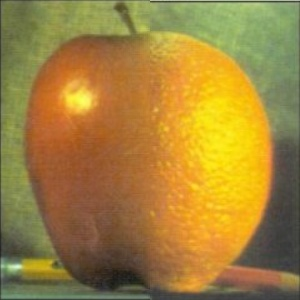
\includegraphics[width=0.9\linewidth]{output/blending1.jpg}
  \caption{Space domain blending}
\end{subfigure}%
\begin{subfigure}{0.5\textwidth}
  \centering
  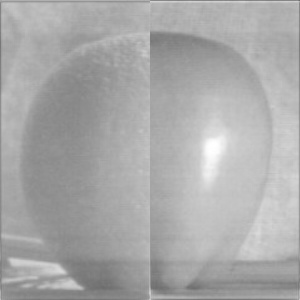
\includegraphics[width=0.9\linewidth]{output/left_right1.jpg}
  \caption{Frequency domain blending}
\end{subfigure}%
\caption{Blending comparison}
\label{fig:comparison-blending}
\end{figure}


